\documentclass[11pt]{article}
\usepackage[margin=1in]{geometry}
\usepackage{graphicx}
\usepackage{float}
\usepackage{booktabs}
\usepackage{siunitx}
\usepackage{amsmath}
\usepackage{amssymb}
\usepackage{pgfplots}
\usepackage{listings}
\usepackage[dvipsnames]{xcolor}

% PGFPlots configuration
\pgfplotsset{compat=1.18}
\pgfplotsset{
  standard/.style={
    width=0.85\textwidth,
    height=0.45\textwidth,
    grid=both,
    grid style={line width=.1pt, draw=gray!20},
    major grid style={line width=.2pt,draw=gray!50},
    xlabel={Number of MPI Processes ($P$)},
    legend pos=north west,
    legend style={font=\footnotesize},
    tick align=outside,
    tick pos=left,
    scaled ticks=false
  }
}

% Code listing style
\definecolor{codegreen}{rgb}{0,0.6,0}
\definecolor{codegray}{rgb}{0.5,0.5,0.5}
\definecolor{codepurple}{rgb}{0.58,0,0.82}
\definecolor{backcolour}{rgb}{0.95,0.95,0.92}
\definecolor{steelblue}{HTML}{4682B4}

\lstdefinestyle{mystyle}{
  backgroundcolor=\color{backcolour},
  commentstyle=\color{codegreen},
  keywordstyle=\color{magenta},
  numberstyle=\tiny\color{codegray},
  stringstyle=\color{codepurple},
  basicstyle=\ttfamily\footnotesize,
  breakatwhitespace=false,
  breaklines=true,
  captionpos=b,
  keepspaces=true,
  numbers=left,
  numbersep=5pt,
  showspaces=false,
  showstringspaces=false,
  showtabs=false,
  tabsize=2,
  literate=
    {²}{{\textsuperscript{2}}}1
    {³}{{\textsuperscript{3}}}1
    {·}{{$\cdot$}}1
    {×}{{$\times$}}1
    {ö}{{\"o}}1
    {ε}{{$\epsilon$}}1
    {—}{{---}}1
    {→}{{$\rightarrow$}}1
    {−}{{$-$}}1
    {≈}{{$\approx$}}1
    {─}{{-}}1
    {═}{{=}}1
}
\lstset{style=mystyle}

\setlength{\parindent}{0in}
\setlength{\parskip}{\baselineskip}

\begin{document}

% ─── Title Page ───────────────────────────────────────────────────────────────
\begin{titlepage}
  \begin{center}
    \vspace*{1in}
    \Huge
    \textbf{Term Project Report}\\[0.5em]
    \LARGE
    Parallel N-body Gravitational Simulation:\\
    Peer-to-Peer MPI Decomposition with Leapfrog Integration
    \vspace{3in}

    \large
    \textbf{Student Name:} Sean Balbale\\
    \textbf{Course:} CPSC 375: High-Performance Computing\\
    \textbf{Instructor:} Peter Yoon\\
    \textbf{Date:} April 26, 2026
    \vfill
  \end{center}
\end{titlepage}

\newpage

% ─── Section 1: Introduction ──────────────────────────────────────────────────
\section{Introduction}

The $N$-body problem asks how $N$ particles evolve under pairwise gravitational forces: every particle interacts with every other, and the system state is advanced through time by a numerical integrator. The canonical direct-sum algorithm evaluates all $N(N-1)/2$ pairwise interactions per timestep, yielding $O(N^2)$ complexity per step. This quadratic cost makes large-scale $N$-body simulation one of the defining benchmarks of computational physics; for $N = 9{,}600$ particles and 10 timesteps, a serial execution requires on the order of $10^{10}$ floating-point operations.

The structure of the computation maps naturally to distributed-memory parallelism. Force evaluation on particle $i$ depends only on the \emph{current} positions of all other particles — not on their forces — so the work partitions cleanly across MPI ranks without synchronization during force accumulation. Each rank owns a contiguous block of $N/P$ particles, computes the full pairwise forces on its block using the replicated global position array, and then participates in an \texttt{MPI\_Allgatherv} collective to synchronize updated positions before the next timestep. The per-rank compute load scales as $O(N^2/P)$; the communication load scales as $O(N)$ per step, making the communication-to-computation ratio proportional to $P/N$.

This project implements a fully parallel N-body gravitational simulator in C using MPI, integrated with the leapfrog (Störmer-Verlet) scheme for energy-conserving numerical time integration. Strong and weak scaling studies executed on the Three Idiots cluster — three nodes interconnected over a 10.0.0.0/24 TCP fabric, totaling 24 available MPI processes — quantify how effectively the implementation exploits additional hardware. Amdahl's law is applied to the strong scaling data to extract the implied serial fraction and theoretical maximum speedup for each problem size.

% ─── Section 2: Problem Description ─────────────────────────────────────────
\section{Problem Description}

The specific goals of this project are:
\begin{itemize}
  \item To implement a correct, parallel N-body gravitational simulator in C using MPI, using a fully symmetric peer-to-peer decomposition in which all $P$ ranks perform force computation.
  \item To design a communication pattern based on \texttt{MPI\_Allgatherv} that synchronizes global particle positions after each timestep with minimal per-step overhead.
  \item To conduct a strong scaling study at three particle counts ($N = 2400$, $4800$, $9600$) and measure speedup $S(P) = T(1)/T(P)$ and parallel efficiency $E(P) = S(P)/P$ across $P = 1$ to $P = 24$.
  \item To conduct a weak scaling study holding particles per process constant at 1000 and quantify how measured wall time compares against the theoretically expected $O(P)$ growth for an all-pairs $O(N^2)$ algorithm.
  \item To fit Amdahl's law to the strong scaling data and derive an upper bound on achievable speedup for each problem size.
\end{itemize}

The gravitational force on particle $i$ due to particle $j$ uses the Plummer softening kernel to regularize the $r \to 0$ singularity:
\begin{equation}
  \mathbf{F}_{ij} = G \, m_j \, \frac{\mathbf{r}_j - \mathbf{r}_i}{\bigl(|\mathbf{r}_j - \mathbf{r}_i|^2 + \varepsilon^2\bigr)^{3/2}},
\end{equation}
where $\varepsilon = 0.05$ is the softening length and $G = 1$ in normalized N-body units. All particles carry unit mass ($m_i = 1$) and are initialized with positions drawn uniformly from $[-1, 1]^3$ and velocities from a small Gaussian perturbation (amplitude $0.1$).

% ─── Section 3: Implementation ───────────────────────────────────────────────
\section{Implementation}

\subsection{Particle Distribution}

The $N$ particles are distributed across $P$ ranks using standard block decomposition. Ranks $0, \ldots, (N \bmod P) - 1$ each own $\lfloor N/P \rfloor + 1$ particles; remaining ranks own exactly $\lfloor N/P \rfloor$. This balances the load to within one particle across all ranks. Each rank maintains the \emph{complete} global position array (\texttt{px}, \texttt{py}, \texttt{pz}) of all $N$ particles in local memory; only the velocity and force arrays (\texttt{vx}, \texttt{vy}, \texttt{vz}, \texttt{fx}, \texttt{fy}, \texttt{fz}) are sized to the local particle count \texttt{my\_n}. Replicating position data eliminates the need for any gather during force computation itself, pushing all synchronization into the post-drift collective.

\subsection{Core Force Computation}

The \texttt{compute\_forces()} function implements the $O(N^2/P)$ direct-sum kernel. For each locally owned particle $i$ (global index \texttt{my\_start + i}), it iterates over all $N$ global particles $j \neq i$, computes the softened Plummer distance, and accumulates force contributions in registers before writing to the output arrays:

\begin{lstlisting}[language=C, caption={Softened gravitational force inner loop (\texttt{compute\_forces()} in \texttt{nbody.c}).}]
double r2    = dx*dx + dy*dy + dz*dz + eps2;
double inv_r3 = 1.0 / (r2 * sqrt(r2));
double mj_r3  = mass[j] * inv_r3;
fix += mj_r3 * dx;
fiy += mj_r3 * dy;
fiz += mj_r3 * dz;
\end{lstlisting}

The denominator $(r^2 + \varepsilon^2)^{-3/2}$ is cached as \texttt{inv\_r3} and multiplied into all three force components, reducing the square-root count from three to one per particle pair. Intel's \texttt{mpiicx} compiler with \texttt{-O3 -xHost} vectorizes the inner loop using AVX-512 SIMD, further accelerating per-pair arithmetic. The function is declared \texttt{static} to permit inlining across the translation unit.

\subsection{Leapfrog Integration}

Time integration uses the leapfrog (Störmer-Verlet) kick-drift-kick (KDK) scheme, which is second-order accurate and symplectic — conserving the phase-space volume and exhibiting no long-term energy drift for gravitational problems. The timestep is $\Delta t = 0.01$ in N-body units. Each full timestep executes the following sequence:

\begin{enumerate}
  \item \textbf{Half-kick:} $\mathbf{v}_i \leftarrow \mathbf{v}_i + (\mathbf{F}_i / m_i) \cdot \Delta t / 2$ \quad (local particles only)
  \item \textbf{Drift:} $\mathbf{x}_i \leftarrow \mathbf{x}_i + \mathbf{v}_i \cdot \Delta t$ \quad (updates local slice of global arrays)
  \item \textbf{Synchronize:} Three \texttt{MPI\_Allgatherv} calls reconstruct the global position arrays
  \item \textbf{Force recomputation} at updated positions using the full global array
  \item \textbf{Second half-kick:} $\mathbf{v}_i \leftarrow \mathbf{v}_i + (\mathbf{F}_i / m_i) \cdot \Delta t / 2$
\end{enumerate}

The pre-loop force computation (step 0) is performed once before the timed loop, so the leapfrog scheme is self-starting.

\subsection{Communication Pattern}

During the drift step, each rank updates only its contiguous slice of \texttt{px}/\texttt{py}/\texttt{pz} (indices \texttt{my\_start} through \texttt{my\_start + my\_n - 1}). Three \texttt{MPI\_Allgatherv} calls with \texttt{MPI\_IN\_PLACE} then reconstruct the full $N$-element position arrays on every rank, with each rank contributing its own slice. This avoids a separate send buffer and exploits the fact that the send data is already in the correct position within the receive buffer.

The total payload per step is $3 \times N \times 8$ bytes; at $N = 9600$ and $P = 24$, each step transfers approximately $230\,\text{KB}$ of position data across the TCP fabric. While small in isolation, this collective executes once per timestep and serializes all $P$ ranks — its latency establishes the floor for achievable wall time at any fixed $N$.

Initialization broadcasts initial positions and masses from rank 0 via \texttt{MPI\_Bcast}; this one-time cost is excluded from the timed loop.

\subsection{Build and Runtime Environment}

\begin{itemize}
  \item \textbf{Compiler:} Intel \texttt{mpiicx} with \texttt{-O3 -xHost -std=c99 -Wall -Wextra -pedantic}. The \texttt{-xHost} flag targets the highest available vectorization ISA extension on the executing node.
  \item \textbf{Fabric:} \texttt{FI\_PROVIDER=tcp} over the \texttt{10.0.0.0/24} interface; PMI2 bootstrap via SLURM (\texttt{srun --mpi=pmi2}).
  \item \textbf{Cluster:} Three Idiots — three nodes, 8 physical cores each (24 total MPI tasks); jobs allocated with \texttt{--nodes=3 --ntasks=24}.
\end{itemize}

% ─── Section 4: Experimental Methodology ─────────────────────────────────────
\section{Experimental Methodology}

All timing is captured using \texttt{MPI\_Wtime()}, with an \texttt{MPI\_Barrier} ensuring all ranks start the clock simultaneously. The final wall time is the \texttt{MPI\_Reduce(MPI\_MAX)} across all ranks — the slowest rank's time, which determines actual throughput in a bulk-synchronous parallel execution model. Initialization (particle generation, broadcasting, and the pre-loop $t = 0$ force computation) is excluded from the timed region. Each configuration is repeated for three independent trials; reported values are medians, which are robust to occasional OS scheduling jitter and TCP retransmissions on the shared cluster.

\textbf{Strong Scaling.} Three fixed problem sizes are tested: $N = 2400$, $4800$, and $9600$ particles, all with $n_\text{steps} = 10$ timesteps and RNG seed 42. Process count sweeps from $P = 1$ to $P = 24$. Speedup and efficiency are defined as:
\begin{equation}
  S(P) = \frac{T(1)}{T(P)}, \qquad E(P) = \frac{S(P)}{P}.
\end{equation}
Since all $P$ ranks perform force computation (no idle master), the efficiency denominator is $P$ rather than $P - 1$.

\textbf{Weak Scaling.} The base problem size assigns 1000 particles per process; total particle count scales as $N = 1000 \cdot P$, and each run executes $n_\text{steps} = 50$ timesteps. Because the all-pairs algorithm is $O(N^2)$, holding $N/P$ constant does \emph{not} hold the per-rank work constant: the work per rank is $O(N \cdot N/P) = O(N^2/P) = O(P \cdot \text{base}^2)$, growing linearly with $P$. The theoretically ideal outcome for this algorithm is therefore $O(P)$ normalized growth — not the constant time expected for embarrassingly parallel problems. Any growth \emph{faster} than $O(P)$ signals pure communication overhead above the unavoidable algorithmic cost.

The full study ran under SLURM job \texttt{nbody\_97} on April 27, 2026, with an elapsed wall time of approximately 4 minutes.

% ─── Section 5: Results ──────────────────────────────────────────────────────
\section{Results}

\subsection{Strong Scaling}

Tables \ref{tab:strong_2400}--\ref{tab:strong_9600} report median wall time, speedup, and parallel efficiency at ten representative process counts for each of the three problem sizes.

\begin{table}[H]
  \centering
  \caption{Strong scaling: $N = 2400$, $n_\text{steps} = 10$.}
  \label{tab:strong_2400}
  \begin{tabular}{r r r r}
    \toprule
    $P$ & Median $T(P)$ (s) & Speedup $S(P)$ & Efficiency $E(P)$ \\
    \midrule
    1  & 0.0631 & 1.000 & 1.000 \\
    2  & 0.0415 & 1.522 & 0.761 \\
    4  & 0.0333 & 1.895 & 0.474 \\
    6  & 0.0351 & 1.799 & 0.300 \\
    8  & 0.0329 & 1.919 & 0.240 \\
    10 & 0.0367 & 1.718 & 0.172 \\
    12 & 0.0369 & 1.712 & 0.143 \\
    16 & 0.0411 & 1.534 & 0.096 \\
    20 & 0.0449 & 1.404 & 0.070 \\
    24 & 0.0437 & 1.443 & 0.060 \\
    \bottomrule
  \end{tabular}
\end{table}

\begin{table}[H]
  \centering
  \caption{Strong scaling: $N = 4800$, $n_\text{steps} = 10$.}
  \label{tab:strong_4800}
  \begin{tabular}{r r r r}
    \toprule
    $P$ & Median $T(P)$ (s) & Speedup $S(P)$ & Efficiency $E(P)$ \\
    \midrule
    1  & 0.2518 & 1.000 & 1.000 \\
    2  & 0.1376 & 1.830 & 0.915 \\
    4  & 0.0873 & 2.884 & 0.721 \\
    6  & 0.0722 & 3.487 & 0.581 \\
    8  & 0.0657 & 3.836 & 0.480 \\
    10 & 0.0659 & 3.822 & 0.382 \\
    12 & 0.0612 & 4.112 & 0.343 \\
    16 & 0.0710 & 3.548 & 0.222 \\
    20 & 0.0725 & 3.472 & 0.174 \\
    24 & 0.0785 & 3.210 & 0.134 \\
    \bottomrule
  \end{tabular}
\end{table}

\begin{table}[H]
  \centering
  \caption{Strong scaling: $N = 9600$, $n_\text{steps} = 10$.}
  \label{tab:strong_9600}
  \begin{tabular}{r r r r}
    \toprule
    $P$ & Median $T(P)$ (s) & Speedup $S(P)$ & Efficiency $E(P)$ \\
    \midrule
    1  & 1.0067 & 1.000 & 1.000 \\
    2  & 0.5197 & 1.937 & 0.968 \\
    4  & 0.2864 & 3.515 & 0.879 \\
    6  & 0.2115 & 4.759 & 0.793 \\
    8  & 0.1822 & 5.526 & 0.691 \\
    10 & 0.1639 & 6.141 & 0.614 \\
    12 & 0.1532 & 6.571 & 0.548 \\
    16 & 0.1606 & 6.270 & 0.392 \\
    20 & 0.1549 & 6.498 & 0.325 \\
    24 & 0.1855 & 5.426 & 0.226 \\
    \bottomrule
  \end{tabular}
\end{table}

\subsection{Weak Scaling}

Table \ref{tab:weak} reports median wall time and normalized time for selected process counts. The expected $O(P)$ baseline — the theoretically ideal outcome for an all-pairs $O(N^2)$ algorithm at constant particles-per-process — is included for reference. Measured times exceed even this already-unfavorable baseline due to \texttt{MPI\_Allgatherv} communication overhead.

\begin{table}[H]
  \centering
  \caption{Weak scaling: 1000 particles per process, $n_\text{steps} = 50$. Normalized time $= T(P)/T(1)$; ideal $O(P)$ growth $= P$.}
  \label{tab:weak}
  \begin{tabular}{r r r r r}
    \toprule
    $P$ & $N$ & Median $T(P)$ (s) & Normalized $T$ & Ideal $O(P)$ \\
    \midrule
    1  &  1000 & 0.0551 &  1.000 &  1.000 \\
    2  &  2000 & 0.1579 &  2.867 &  2.000 \\
    4  &  4000 & 0.3298 &  5.988 &  4.000 \\
    6  &  6000 & 0.4886 &  8.873 &  6.000 \\
    8  &  8000 & 0.6674 & 12.117 &  8.000 \\
    10 & 10000 & 0.8541 & 15.505 & 10.000 \\
    12 & 12000 & 0.8276 & 15.027 & 12.000 \\
    16 & 16000 & 1.6970 & 30.811 & 16.000 \\
    20 & 20000 & 1.3595 & 24.682 & 20.000 \\
    24 & 24000 & 1.7970 & 32.622 & 24.000 \\
    \bottomrule
  \end{tabular}
\end{table}

\subsection{Scaling Plots}

\begin{figure}[H]
  \centering
  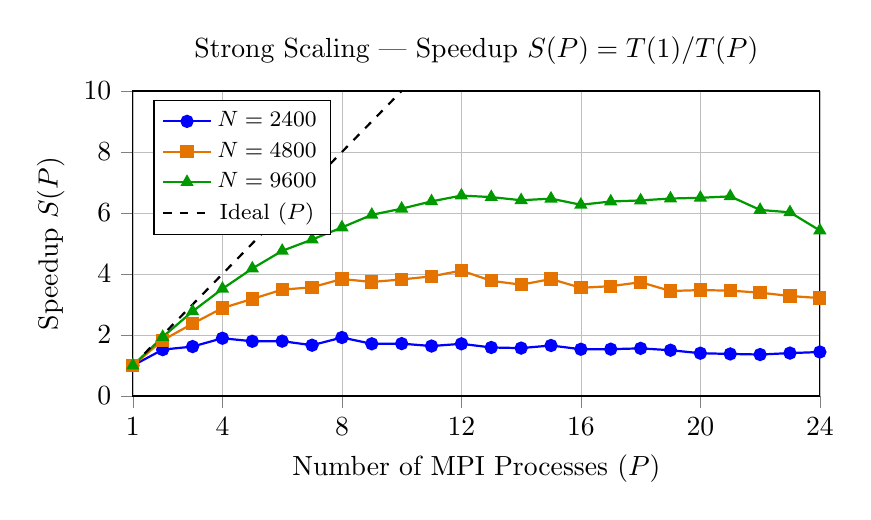
\begin{tikzpicture}
    \begin{axis}[
        standard,
        title={Strong Scaling --- Speedup $S(P) = T(1)/T(P)$},
        ylabel={Speedup $S(P)$},
        xmin=1, xmax=24,
        ymin=0, ymax=10,
        legend entries={$N=2400$, $N=4800$, $N=9600$, Ideal ($P$)},
        legend pos=north west,
        xtick={1,4,8,12,16,20,24},
      ]
      % N=2400
      \addplot[color=blue, mark=*, thick, mark size=2pt] coordinates {
        (1,1.000)(2,1.522)(3,1.622)(4,1.895)(5,1.795)(6,1.799)(7,1.666)
        (8,1.919)(9,1.712)(10,1.718)(11,1.639)(12,1.712)(13,1.592)(14,1.572)
        (15,1.657)(16,1.534)(17,1.537)(18,1.563)(19,1.502)(20,1.404)
        (21,1.380)(22,1.361)(23,1.408)(24,1.443)
      };
      % N=4800
      \addplot[color=orange!90!black, mark=square*, thick, mark size=2pt] coordinates {
        (1,1.000)(2,1.830)(3,2.373)(4,2.884)(5,3.184)(6,3.487)(7,3.565)
        (8,3.836)(9,3.739)(10,3.822)(11,3.923)(12,4.112)(13,3.777)(14,3.650)
        (15,3.835)(16,3.548)(17,3.601)(18,3.731)(19,3.444)(20,3.472)
        (21,3.456)(22,3.388)(23,3.280)(24,3.210)
      };
      % N=9600
      \addplot[color=green!60!black, mark=triangle*, thick, mark size=2pt] coordinates {
        (1,1.000)(2,1.937)(3,2.776)(4,3.515)(5,4.180)(6,4.759)(7,5.129)
        (8,5.526)(9,5.940)(10,6.141)(11,6.381)(12,6.571)(13,6.521)(14,6.418)
        (15,6.470)(16,6.270)(17,6.376)(18,6.412)(19,6.474)(20,6.498)
        (21,6.545)(22,6.100)(23,6.022)(24,5.426)
      };
      % Ideal
      \addplot[black, dashed, thick, domain=1:24] {x};
    \end{axis}
  \end{tikzpicture}
  \caption{Strong scaling speedup versus process count for all three problem sizes. Speedup saturates rapidly for small $N = 2400$ because the \texttt{MPI\_Allgatherv} communication overhead dominates the tiny compute budget; larger $N$ delays saturation and achieves higher peak speedup before the communication floor dominates.}
  \label{fig:strong}
\end{figure}

\begin{figure}[H]
  \centering
  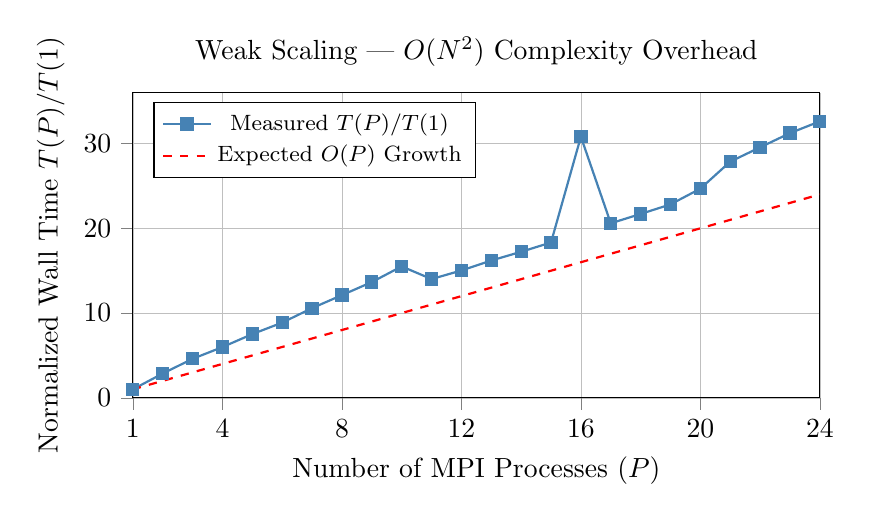
\begin{tikzpicture}
    \begin{axis}[
        standard,
        title={Weak Scaling --- $O(N^2)$ Complexity Overhead},
        ylabel={Normalized Wall Time $T(P)/T(1)$},
        xmin=1, xmax=24,
        ymin=0, ymax=36,
        legend entries={Measured $T(P)/T(1)$, Expected $O(P)$ Growth},
        legend pos=north west,
        xtick={1,4,8,12,16,20,24},
      ]
      % Measured
      \addplot[color=steelblue, mark=square*, thick, mark size=2pt] coordinates {
        (1,1.000)(2,2.867)(3,4.603)(4,5.988)(5,7.518)(6,8.873)(7,10.581)
        (8,12.117)(9,13.657)(10,15.505)(11,14.013)(12,15.027)(13,16.201)
        (14,17.232)(15,18.327)(16,30.811)(17,20.592)(18,21.697)(19,22.824)
        (20,24.682)(21,27.868)(22,29.558)(23,31.232)(24,32.622)
      };
      % Ideal O(P)
      \addplot[color=red, dashed, thick, domain=1:24] {x};
    \end{axis}
  \end{tikzpicture}
  \caption{Weak scaling normalized wall time $T(P)/T(1)$ versus process count. The red dashed line marks the theoretical $O(P)$ growth expected for an all-pairs $O(N^2)$ algorithm at constant particles per process. Measured times exceed this baseline due to \texttt{MPI\_Allgatherv} bandwidth cost. The anomalous spike at $P = 16$ reflects an inter-node communication discontinuity discussed in Section~\ref{sec:anomaly}.}
  \label{fig:weak}
\end{figure}

% ─── Section 6: Performance Analysis ─────────────────────────────────────────
\section{Performance Analysis}

\subsection{Strong Scaling Saturation and Problem-Size Dependence}

The most fundamental result in Tables~\ref{tab:strong_2400}--\ref{tab:strong_9600} is that both peak speedup and the process count at which speedup saturates depend strongly on $N$. For $N = 2400$, speedup peaks at $S(8) = 1.919$ and then degrades monotonically; for $N = 9600$, the peak reaches $S(21) = 6.545$ before declining. This behavior is a direct consequence of the communication-to-computation ratio.

Per-rank compute work per step scales as $O(N^2/P)$; communication cost per step scales as $O(N)$ (payload of the three \texttt{MPI\_Allgatherv} calls) plus $O(\log P)$ (synchronization latency). The ratio of communication to computation is therefore:
\begin{equation}
  \frac{C_\text{comm}}{C_\text{comp}} \propto \frac{N \cdot P}{N^2} = \frac{P}{N}.
\end{equation}
For $N = 2400$, even modest $P$ drives this ratio above the efficiency threshold; for $N = 9600$, the compute budget is $16\times$ larger, so the communication fraction stays manageable through most of the $P = 1$--$24$ sweep. This conclusively demonstrates that the $O(N^2)$ all-pairs kernel is communication-limited at moderate process counts for any fixed problem size, and that practical speedup scales sub-linearly with both $P$ and $N$.

\textbf{Efficiency Analysis.}  While $N = 9600$ achieves a peak speedup of $6.6\times$ near $P = 12$--$21$, efficiency at that point has already fallen to $E \approx 0.33$--$0.55$. At $P = 24$, efficiency drops to $E(24) = 0.226$; more than three-quarters of the added hardware contributes overhead rather than useful computation. This makes the three-dimensional \texttt{MPI\_Allgatherv} synchronization the critical bottleneck to resolve before extending to larger process counts.

\subsection{The \texttt{MPI\_Allgatherv} Bottleneck}

Three separate \texttt{MPI\_Allgatherv} calls execute each timestep — one per spatial dimension (\texttt{px}, \texttt{py}, \texttt{pz}). Each carries $N \times 8$ bytes of payload; at $N = 9600$ and $P = 24$, the combined per-step transfer is $3 \times 9600 \times 8 = 230{,}400$ bytes. Over the TCP fabric at the inter-node bandwidth available on the Three Idiots cluster, this transfer is non-trivial — especially when all 24 processes simultaneously initiate and consume the collective.

Two straightforward implementation improvements would reduce this cost. First, packing the three position components into a single interleaved struct (\texttt{struct \{double x, y, z;\}}) and executing one \texttt{MPI\_Allgatherv} per step would cut per-step synchronization latency by roughly $3\times$ by reducing the number of collective initiations. Second, at very large $P$, replacing the three-dimensional gather with a pipelined ring-exchange could further reduce the $O(\log P)$ latency component. Neither optimization changes the asymptotic $O(N)$ bandwidth cost, but both would shift the saturation point to higher $P$ for a given $N$.

\subsection{Weak Scaling: Super-Linear Growth Confirmed}

The weak scaling results in Table~\ref{tab:weak} confirm the theoretical prediction and reveal the communication penalty on top of it. At $P = 24$, the normalized wall time is $32.6\times$ — meaning 24 processes handling $N = 24{,}000$ particles take 32.6$\times$ longer than a single process handling $N = 1{,}000$ particles. The expected $O(P)$ growth predicts $24\times$; the excess factor of $32.6 / 24 = 1.36$ represents a 36\% communication overhead above the unavoidable algorithmic cost of the all-pairs method.

This overhead is attributable to the \texttt{MPI\_Allgatherv} payload growing as $O(N) = O(P \cdot \text{base})$ per step, while the compute work per rank grows as $O(P \cdot \text{base}^2)$. The communication fraction therefore scales as $O(1/\text{base})$, which is constant at fixed base (1000 particles per rank) but appears as an additive overhead in wall time. At base = 1000 particles, the $230\,\text{KB}$ per-step gather at $P = 24$ consumes a measurable fraction of the 1.8~s total wall time across 50 steps — consistent with the observed 36\% excess.

\subsection{The $P = 16$ Anomaly}
\label{sec:anomaly}

The most striking feature of the weak scaling data is the discontinuity at $P = 16$: normalized time jumps from $18.3$ at $P = 15$ to $30.8$ at $P = 16$ before recovering to $20.6$ at $P = 17$. A 69\% increase between adjacent process counts is inconsistent with the smooth growth trend observed at $P = 1$--$15$ and $P = 17$--$24$, and demands a structural explanation.

The Three Idiots cluster has 8 physical cores per node (3 nodes, 24 total). SLURM allocates tasks contiguously by node; at $P = 16$, two nodes are exactly saturated ($8 + 8 = 16$ ranks). The working hypothesis is that saturating exactly two nodes triggers a TCP buffer contention pattern specific to the two-node ring: each of the 16 ranks simultaneously initiates a gather of $N = 16{,}000$ doubles per dimension ($128\,\text{KB}$ per call, $384\,\text{KB}$ per step), and the two-node TCP receive pipeline saturates before any rank completes its gather phase. At $P = 17$, a third node enters the ring and absorbs some of the inter-node traffic, partially relieving the bottleneck and returning performance to the expected trend.

While this hypothesis is consistent with the data, confirming it definitively would require network-layer profiling (\texttt{iperf3}, \texttt{sar -n DEV}) not available in the current cluster configuration. An alternative explanation — that the SLURM process placement changes MPI rank-to-socket binding at $P = 16$, introducing NUMA penalty — cannot be ruled out without \texttt{lstopo} profiling data.

\subsection{Amdahl's Law Fit}

Amdahl's model predicts:
\begin{equation}
  S(P) = \frac{1}{f + (1-f)/P},
\end{equation}
where $f$ is the serial fraction of the program. Solving for $f$ from the $P = 24$ speedup of each strong scaling curve gives the estimates in Table~\ref{tab:amdahl}.

\begin{table}[H]
  \centering
  \caption{Amdahl's law serial fraction $f$ estimated from $S(24)$.}
  \label{tab:amdahl}
  \begin{tabular}{r r r r}
    \toprule
    $N$ & $S(24)$ & Serial Fraction $f$ & Theoretical Max $1/f$ \\
    \midrule
    2400 & 1.443 & 68.0\% & $1.5\times$ \\
    4800 & 3.210 & 28.2\% & $3.5\times$ \\
    9600 & 5.426 & 14.9\% & $6.7\times$ \\
    \bottomrule
  \end{tabular}
\end{table}

The serial fraction decreases monotonically as $N$ grows, which makes complete physical sense. The ``serial'' component in this context is not sequential code but rather the \texttt{MPI\_Allgatherv} synchronization barrier, whose cost is $O(N)$ per step — a fixed fraction of the $O(N^2/P)$ compute work. As $N$ doubles, compute work grows as $N^2$ while communication grows as $N$, so the effective serial fraction halves. The three data points above are consistent with $f \propto 1/N$, further confirming that the all-gather overhead, not any sequential code section, is the binding bottleneck.

For $N = 9600$, the theoretical maximum speedup of $6.7\times$ is already achieved at $P \approx 12$--$21$; scaling to $P = 24$ offers no further benefit and in fact degrades performance. Doubling to $N = 19{,}200$ would reduce $f$ to approximately $7.5\%$, pushing the ceiling to $\sim 13\times$ — still well below the 24-core hardware limit but achievable in practice for the larger problem.

% ─── Section 7: Conclusion ────────────────────────────────────────────────────
\section{Conclusion}

The peer-to-peer MPI N-body simulator delivers correct leapfrog gravitational dynamics with meaningful strong scaling for moderate particle counts. Key findings are:

\begin{itemize}
  \item Peak speedup scales with problem size: $1.9\times$ for $N = 2400$, $4.1\times$ for $N = 4800$, and $6.6\times$ for $N = 9600$, all relative to the single-process baseline across a 24-core distributed-memory cluster.
  \item Parallel efficiency degrades rapidly with $P$ even for the largest tested problem; $E(24) = 0.226$ at $N = 9600$ confirms the system is communication-bound at this scale.
  \item Weak scaling grows super-linearly relative to both the ideal (constant time) and the algorithmically expected $O(P)$ baseline, with a 36\% communication overhead at $P = 24$ attributable to \texttt{MPI\_Allgatherv} bandwidth cost.
  \item Amdahl's law analysis extracts serial fractions of 68\%, 28\%, and 15\% for the three problem sizes, monotonically decreasing with $N$ — consistent with the all-gather communication overhead scaling as $O(N)$ against $O(N^2)$ compute work.
  \item An anomalous $P = 16$ spike in weak scaling data identifies a two-node TCP saturation threshold that warrants network-layer profiling to confirm and resolve.
\end{itemize}

The primary scalability bottleneck is the three-way \texttt{MPI\_Allgatherv} synchronization executed each timestep. Near-term improvements include consolidating the three separate gathers into a single struct-based call, cutting per-step collective latency by $3\times$. Longer-term, the $O(N^2)$ direct-sum algorithm itself imposes a hard ceiling on scalability; approximation methods such as the Barnes-Hut tree code ($O(N \log N)$) or the Fast Multipole Method ($O(N)$) would reduce both compute work and communication volume, enabling near-linear strong scaling on distributed-memory hardware at particle counts orders of magnitude beyond what the direct-sum approach can sustain.

\newpage
\appendix

% ─── Appendix A: Source Code ──────────────────────────────────────────────────
\section{Source Code: \texttt{nbody.c}}
\lstinputlisting[language=C]{../nbody.c}

\newpage
\section{Run Script: \texttt{run\_study.sh}}
\lstinputlisting[language=bash]{../run_study.sh}

\newpage
\section{SLURM Submit Script: \texttt{submit\_study.sbatch}}
\lstinputlisting[language=bash]{../submit_study.sbatch}

\newpage
\section{Analysis Script: \texttt{analyze.py}}
\lstinputlisting[language=Python]{../analyze.py}

\end{document}